% GENERATED by scripts/paper/figures.py -- do not edit by hand.
\begin{figure}[t]
\centering
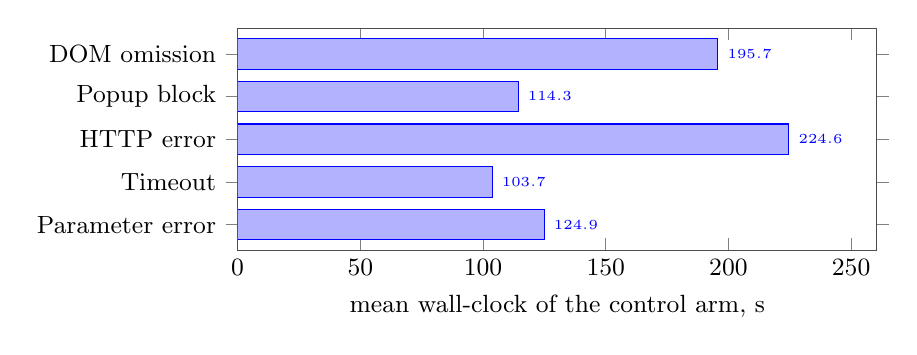
\begin{tikzpicture}
\begin{axis}[
  width=0.8\linewidth, height=4.4cm,
  xbar, bar width=11pt, xmin=0, xmax=260.5,
  ytick={1,2,3,4,5}, y dir=reverse, ymin=0.4, ymax=5.6,
  yticklabels={{DOM omission},{Popup block},{HTTP error},{Timeout},{Parameter error}},
  xlabel={mean wall-clock of the control arm, s},
  tick label style={font=\small}, label style={font=\small},
  nodes near coords, nodes near coords style={font=\tiny},
  fill=gray!55, draw=black!70,
]
\addplot coordinates {(195.7,1) (114.3,2) (224.6,3) (103.7,4) (124.9,5)};
\end{axis}
\end{tikzpicture}
\caption{The noise floor. These five arms are the \emph{same} agent configuration under the clean condition; each is the control half of one fault's pair set. Their means span a factor of 2.17$\times$, so absolute cross-arm timings are dominated by machine-level drift and only within-pair deltas are interpretable.}
\label{fig:noisefloor}
\end{figure}
